%!TeX root = MarquezSalazarBrandon-Tarea04-Reporte.tex
\section{Introduction}
\subsection{Texture (visual) definition}

Described by an article of Sonymage \cite{sonymage_TexturaVisual}, a visual texture refers
to the appearance of an object, and can be given different adjectives such as rough, smooth,
fine, coarse, etc.

For Dan Scott, texture regards the \say{\textit{surface quality}}\cite {drawpaintaVET}.
Also, Dan distinguishes between the physical texture and the illusion of texture.
Where the first one is actual surface properties being appreciable by touch and sight;
and the second only can be appreciated by sight.

Following what Anil wrote in \cite{Jain1988-vs}, \say{the term texture generally refers to
repetition of basic texture elements called \textit{texels}}.

\section{Methods and Materials}
In this experiment, it'll be implemented the SDH algorithm explained in \cite{syT0826}.
To afford this, the library \textbf{OpenCV} will be needed.
The chosen language is \textbf{C++} due it's performance, explicitness and object oriented
structure.
On the other hand, for the experimentation, 4 images will be processed and documented
in this text.

The images to be processed are the following:
\begin{figure}[!h]
  \centering
  \begin{subfigure}[b]{0.48\textwidth}
    \centering
    
\includegraphics[width=\textwidth]{res/Solid.png}
    \caption{Solid.png}
  \end{subfigure}
  \begin{subfigure}[b]{0.48\textwidth}
    \centering
    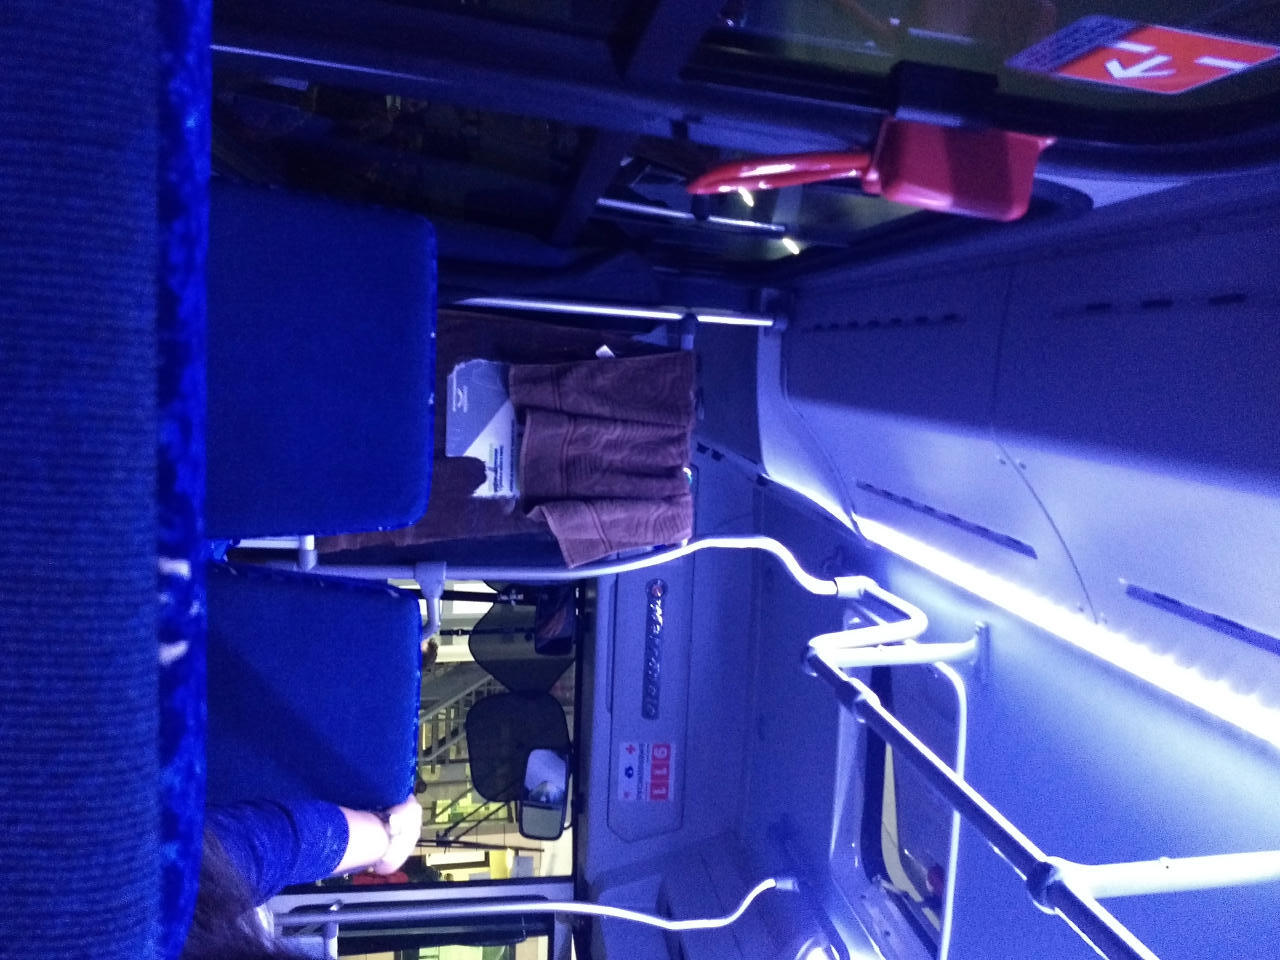
\includegraphics[width=\textwidth]{res/Bus.jpeg}
    \caption{Bus.jpeg}
  \end{subfigure}
  \begin{subfigure}[b]{0.48\textwidth}
    \centering
    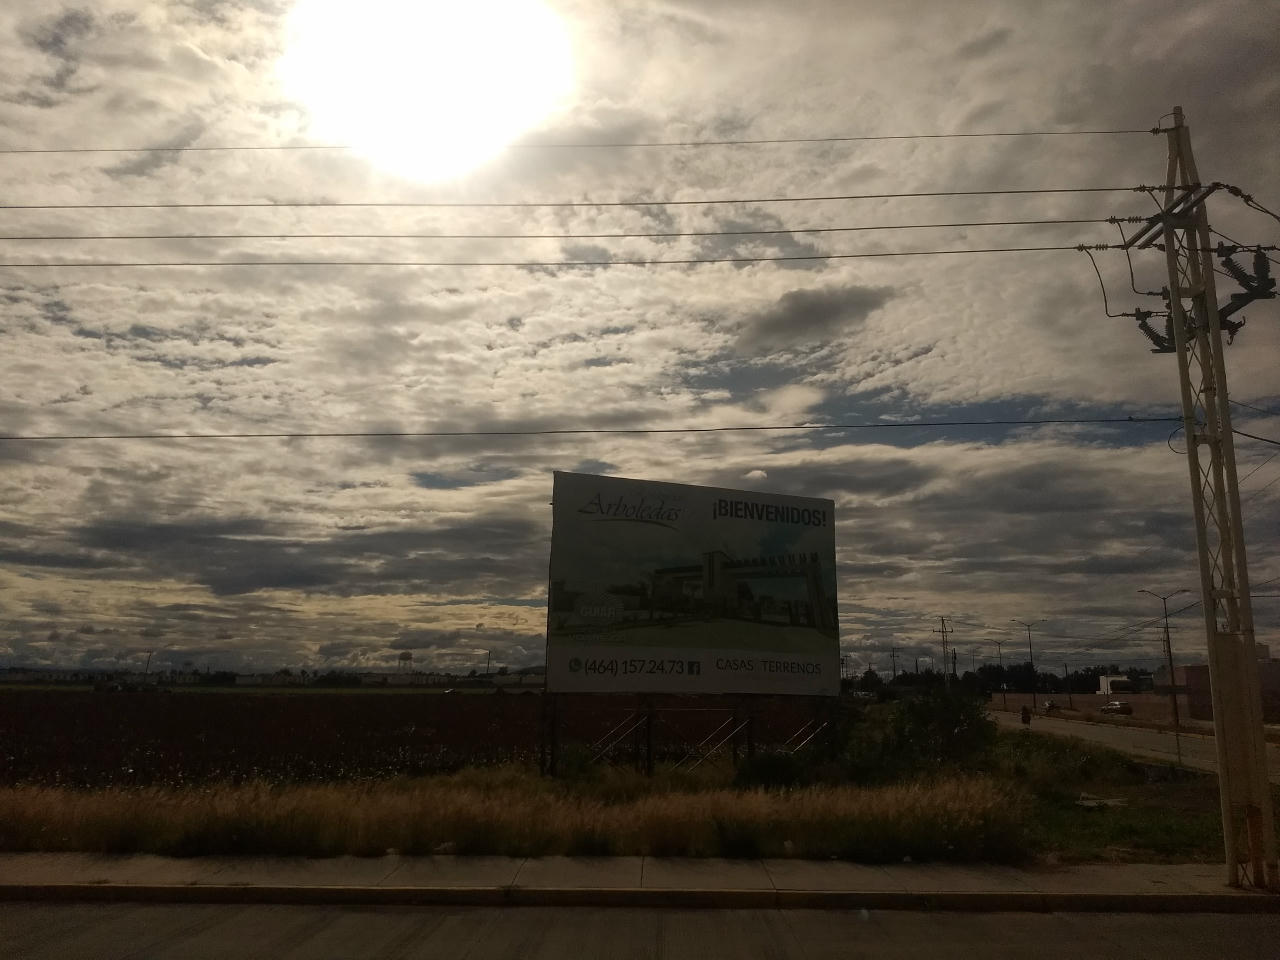
\includegraphics[width=\textwidth]{res/Sunset-cirro.jpeg}
    \caption{Sunset-cirro.jpeg}  
  \end{subfigure}
  \begin{subfigure}[b]{0.48\textwidth}
    \centering
    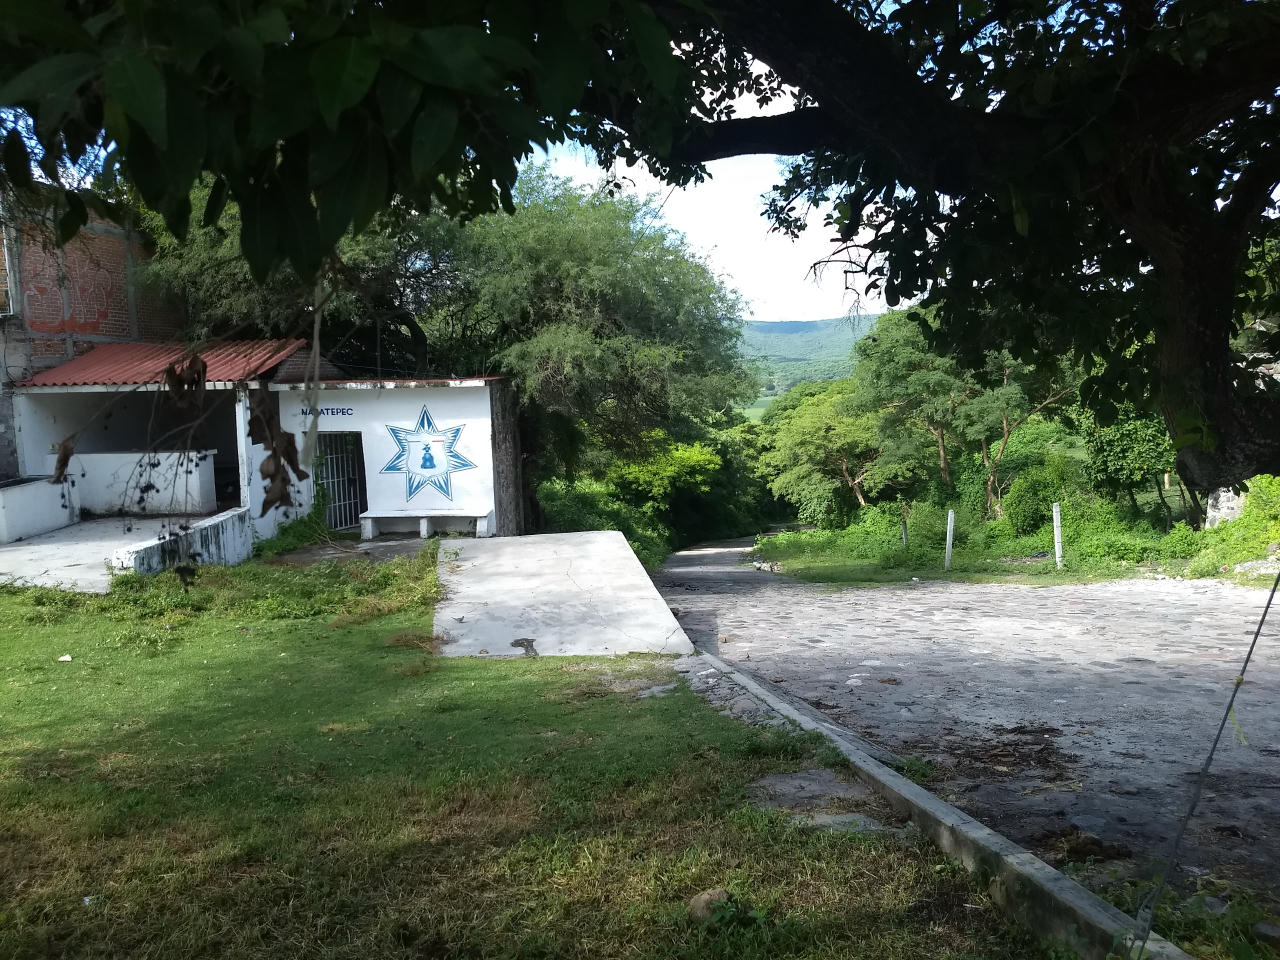
\includegraphics[width=\textwidth]{res/Natur-police.jpeg}
    \caption{Natur-police.jpeg}
  \end{subfigure}

  \caption{Images to be processed\\\tiny{Photos by Lang Lovdog Inu Oókami}}
\end{figure}
